Existen números herramientas de etiquetado compatibles con \textbf{YOLO}, pero quizás una de las más sencillas de usar sea \textit{LabelIMG}. Esta herramienta se encuentra disponible tanto para \textit{Windows} como para \textit{MAC OS/Linux}.\\

Para poder acceder a \textit{LabelIMG} se puede hacer a través de su propio repositorio de \textit{GitHub} \url{https://github.com/heartexlabs/labelImg}, el cual presenta las distintas opciones de instalación que se tienen dependiendo de la plataforma. En caso de necesitar instalarla en un ordenador \textit{MAC OS/Linux}, debido a las diferentes incompatibilidades entre librerías con las que nos encontramos en su momento, recomendamos instalar las que se indican en el fichero de \textbf{requirements.txt}. \\

Para hacer uso de dicha herramienta simplemente debemos inicializar su fichero base, el cual lanzará una interfaz con la que interactuaremos para realizar el etiquetado. Para ello, accediendo a la segunda carpeta de nuestro repositorio denominada \textit{2_Etiquetado}, podremos arrancarla:

\begin{lstlisting}
python3 labelImg.py
\end{lstlisting}

Internamente podemos modificar cuáles queremos que sean las clases que por defecto tenemos para etiquetar, en nuestro caso tenemos las diferentes clases de señales: prohibición, peligro, obligación y otros. Si se quisiera modificarlo porque se fuera a utilizar para otra aplicación, se podría modificar mediante el fichero \textbf{predefined_classes.txt} disponible dentro de la carpeta \textit{data}.\\

Se puede trabajar con una imagen individual o con un conjunto de ellas, a través de los botones indicados a continuación podremos abrir las imágenes:

\begin{figure}[H]
	\centering
	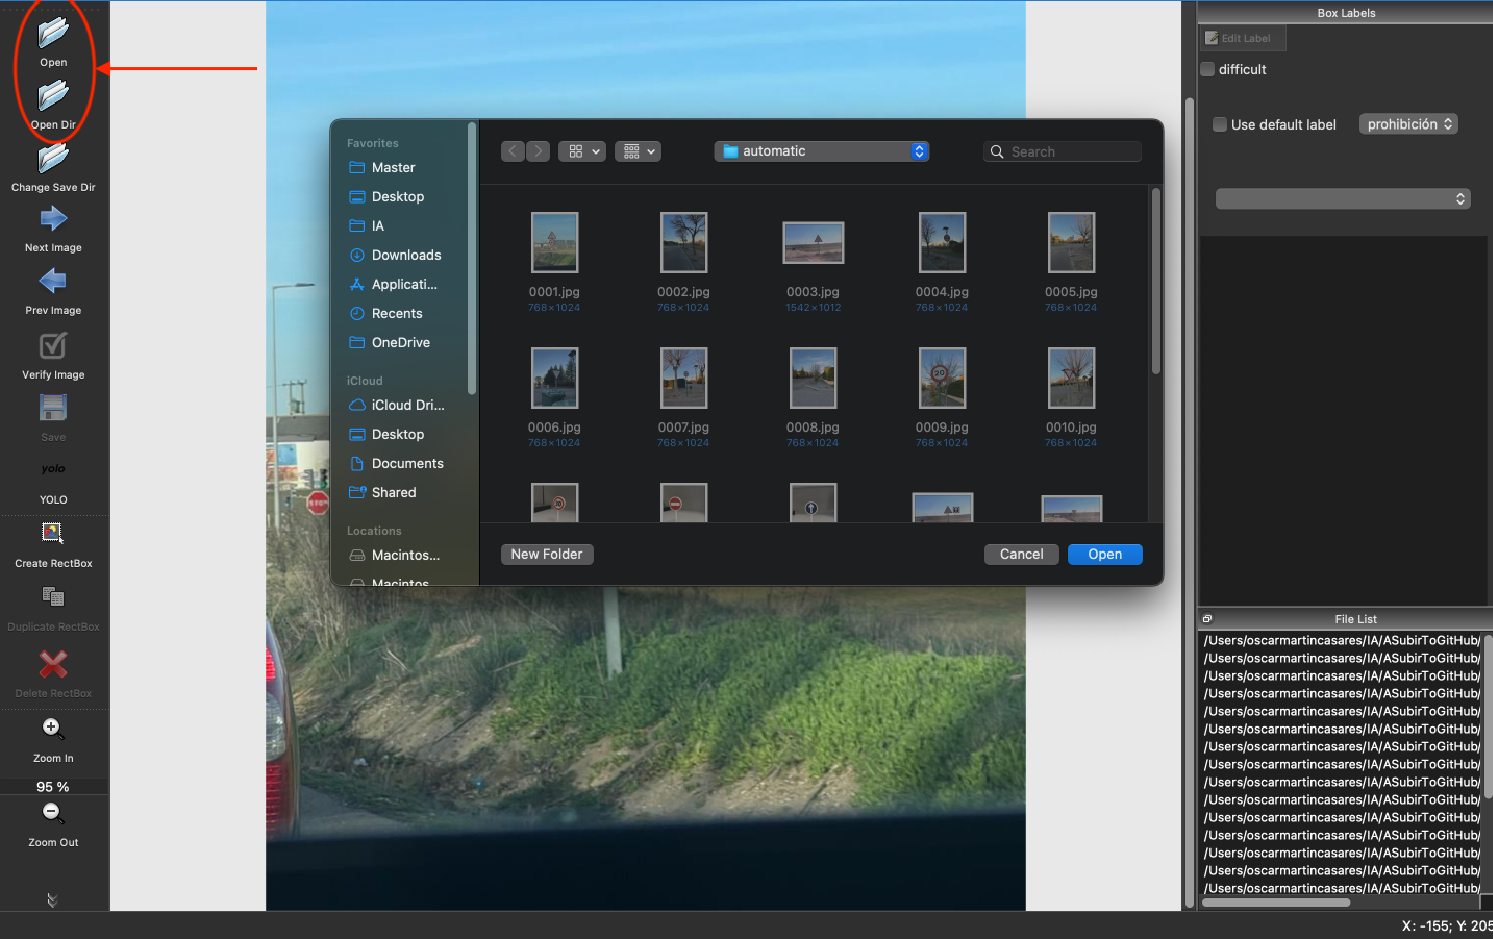
\includegraphics[width=\textwidth]{Imagenes/AnexoI_Manual/AA/etiquetado1.pdf}
	\caption{Etiquetado de una señal}
	\label{etique1}
\end{figure}